\begin{frame}
    \frametitle{Sistema GPS}
    % Página que explica como funciona un GPS http://gutovnik.com/como_func_sist_gps.htm
    % video explicativo: https://youtu.be/U3eX6QKS9kY
    \begin{itemize}
        \item Se toma la distancia a cuatro satélites (uno por cada incógnita: latitud, longitud, altitud y offset en tiempo del del reloj del receptor) y se estima la pose por triangulación.
        \item La distancia se obtiene midiendo el tiempo que tarda en llegar la señal del satélite %emitida por el satélite en llegar hasta nuestro receptor de GPS
        \note{En el caso del GPS estamos midiendo una señal de radio, que sabemos que viaja a la velocidad de la luz, alrededor de 300.000 km por segundo.}
        \note{La señal que recibe un receptor de GPS no es solamente un Código Pseudo Aleatorio con fines de timing. También contiene un mensaje de navegación con información sobre la órbita exacta del satélite}
        \note{Otra manera de manejar los errores inducidos por la atmósfera es comparar la velocidad relativa de dos señales diferentes. Esta medición de doble frecuencia es muy sofisticada y solo es posible en receptores GPS muy avanzados. Estos son los GPS-RTK!}
        \note{Los receptores "normales" basados navegación por satélite, comparan una señal pseudoaleatoria que es enviada desde el satélite con una copia interna generada por la misma señal. Puesto que la senal del satelite tarda tiempo en alcanzar al receptor, las dos senales no se alinean correctamente, la copia del satelite se retrasa en referencia a la copia local. Al retrasar progresivamente la copia local, las dos señales se alinearán correctamente en algún momento. Este retraso es el tiempo necesario para que la señal alcance al receptor, y del resultado de esto puede ser calculada la distancia al satélite. La precisión de la medición resultante es generalmente una función de la capacidad  electrónica del receptor para comparar exactamente las dos señales.}
        \item Fuentes de ruido (Retrasos ionosféricos y atmosféricos, Efecto Multitrayectoria, Dilución de la Precisión, reloj del satélite)
        \item Error de posicionamiento métrico ($\sim$2 m)
    \end{itemize}

    \centering
    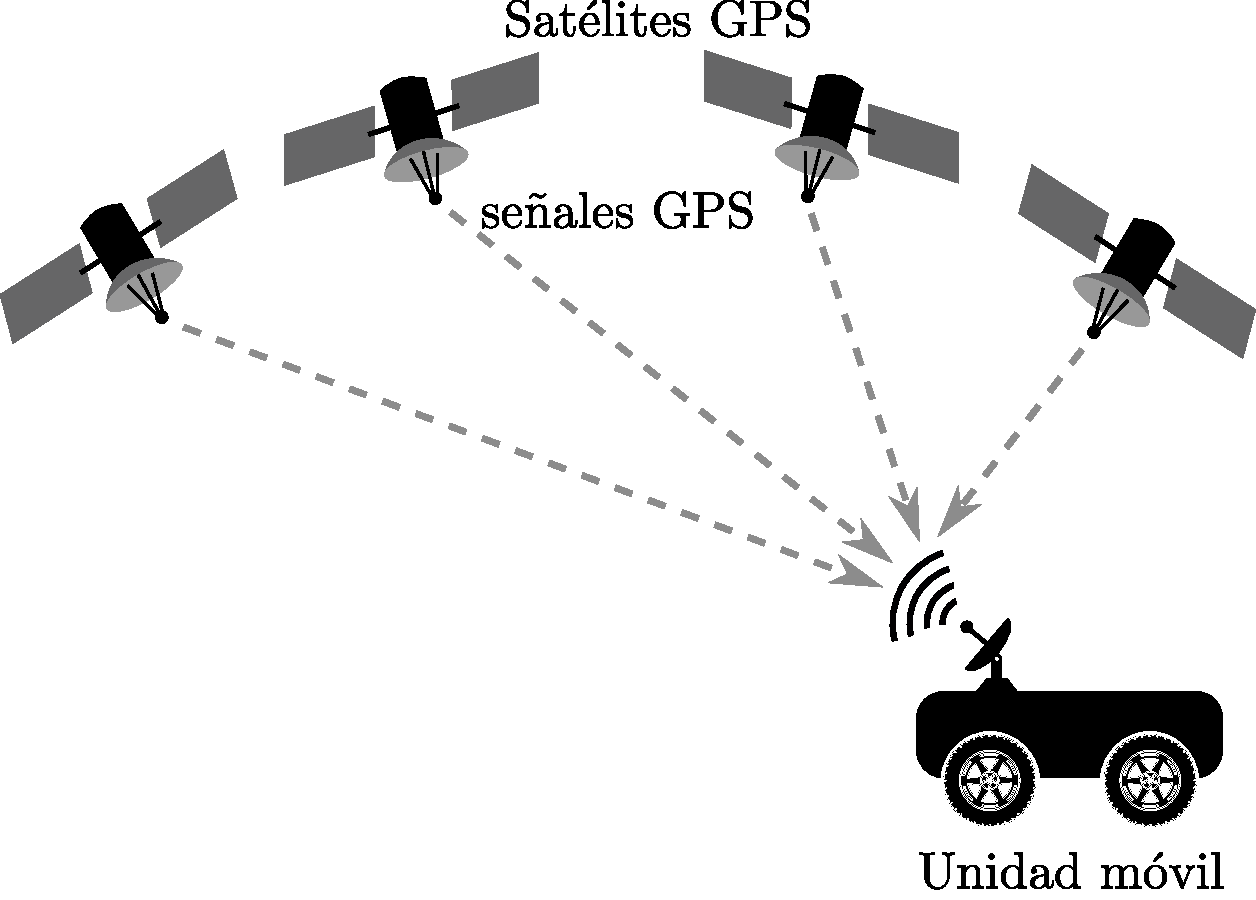
\includegraphics[width=0.5\columnwidth]{gps.pdf}

\end{frame}
